\documentclass{beamer}
  \mode<presentation> {
    \usetheme{Frankfurt}
  }

% \usepackage{times}
\usepackage{amsmath,amssymb}
\usepackage[english]{babel}
\usepackage[utf8]{inputenc}
% \usepackage[latin1]{inputenc}

\usepackage{fancybox}
\usefonttheme[onlymath]{serif}
\boldmath


\usepackage{scalefnt}
\usepackage{ragged2e}
\usepackage{graphics}
\usepackage{url}
\usepackage{graphicx}
\usepackage{mathrsfs}
\usepackage{amsfonts}
\usepackage[authoryear,round]{natbib}

\graphicspath{ {./figures/} }

\def \calE {\mathcal{E}}
\def \calF {\mathcal{F}}
\def \calG {\mathcal{G}}
\def \calN {\mathcal{N}}
\def \calP {\mathcal{P}}
\def \calR {\mathcal{R}}
\def \calW {\mathcal{W}}


\usepackage{array}
\newcolumntype{L}[1]{>{\raggedright\let\newline\\\arraybackslash\hspace{0pt}}m{#1}}
\newcolumntype{C}[1]{>{\centering\let\newline\\\arraybackslash\hspace{0pt}}m{#1}}
\newcolumntype{R}[1]{>{\raggedleft\let\newline\\\arraybackslash\hspace{0pt}}m{#1}}

\beamertemplatenavigationsymbolsempty

%%%%%%%%%%%%%%%%%%%%%%%%%%%%%%%%%%%%%%%%%%%%%%%%%%%%%%%%%%%%%%%%%%%%%%%%%%%%%%%%%%%%%%%%%%%%%%%%%%%%%%%%%%%%
%%%%%%%%%%%%%%%%%%%%%%%%%%%%%%%%%%%%%%%%%%%%%%%%%%%%%%%%%%%%%%%%%%%%%%%%%%%%%%%%%%%%%%%%%%%%%%%%%%%%%%%%%%%%

  \title[Chagas \& Big Data]{Uncovering the Spread of an Infectious
	Disease with Mobile Phone Data}

  \author[Salles,Sarraute,de Monasterio]{Juan de Monasterio\inst{1}
  \and Alejo Salles\inst{1} \\
  \and Carlos Sarraute\inst{3} 
  }
  \institute[]{
  \and \inst{1} Universidad de Buenos Aires
  \and \inst{3} Grandata Labs 

  }

  \date{ FCEyN \\ Diciembre , 2017}


%\setbeamertemplate{footline}[text line]{\bf \insertshortauthor \hfill \insertshorttitle \hfill \insertframenumber/29}
\setbeamertemplate{footline}[text line]{\hfill \insertframenumber / 35}

\AtBeginSection[]
{
  \begin{frame}<beamer>{Agenda}
    \tableofcontents[currentsection]
  \end{frame}
}
  
%%%%%%%%%%%%%%%%%%%%%%%%%%%%%%%%%%%%%%%%%%%%%%%%%%%%%%%%%%%%%%%%%%%%%%%%%%%%%%%%%%%%%%%%%%%%%%%%%%%%%%%%%%%%
%%%%%%%%%%%%%%%%%%%%%%%%%%%%%%%%%%%%%%%%%%%%%%%%%%%%%%%%%%%%%%%%%%%%%%%%%%%%%%%%%%%%%%%%%%%%%%%%%%%%%%%%%%%%
%%%%%%%%%%%%%%%%%%%%%%%%%%%%%%%%%%%%%%%%%%%%%%%%%%%%%%%%%%%%%%%%%%%%%%%%%%%%%%%%%%%%%%%%%%%%%%%%%%%%%%%%%%%%
\begin{document}


\begin{frame}
\titlepage
\end{frame}


%%%%%%%%%%%%%%%%%%%%%%%%%%%%%%%%%%%%%%%%%%%%%%%%%%%%%%%%%%%%%%%%%%%%%%%%%%%%%%%%%%%%%%%%%%%%%%%%%%%%%%%%%%%%
\section{Introducción}
%%%%%%%%%%%%%%%%%%%%%%%%%%%%%%%%%%%%%%%%%%%%%%%%%%%%%%%%%%%%%%%%%%%%%%%%%%%%%%%%%%%%%%%%%%%%%%%%%%%%%%%%%%%%

\begin{frame}{Presentación y Contexto del Proyecto}
	
	\begin{block}{Idea del proyecto}
		\begin{itemize}
			
			\item Comienzo en agosto 2015 
			\item Colaboración entre Fundación Mundo Sano, GranData Labs y UBA
			\item Investigacion sobre la enfermedad del Chagas.
			\item Trabajo multidisciplinario de biologia, computacion, estadistica
			\begin{itemize}
				\item ``Big Data'' + Aprendizaje Automático integrando datos de telefonía celular
				\item  Buscamos caracterizar y predecir migraciones de usuarios
			\end{itemize}
		\end{itemize}
		
	\end{block}
	
	\pause
	
	\begin{block}{ Colaboración}
		\begin{itemize}
			\item Diego Weinberg (Fundación Mundo Sano)
			\item Carlos Sarraute, Carolina Lang (GranData Labs)
			\item Alejo Salles (Instituto de Cálculo, UBA)
		\end{itemize}
	\end{block}
	
\end{frame}

%%%%%%%%%%%%%%%%%%%%%%%%%%%%%%%%%%%%%%%%%%%%%%%%%%%%%%%%%%%%%%%%%%%%%%%%%%%%%%%%%%%%%%%%%%%%%%%%%%%%%%%%%%%%

\begin{frame}{Problemática}
	
	\begin{block}{Idea del proyecto}
		\begin{itemize}
			
			\item Comienzo en agosto 2015 
			\item Colaboración entre Fundación Mundo Sano, GranData Labs y UBA
			\item Investigacion sobre la enfermedad del Chagas.
			\item Trabajo multidisciplinario de biologia, computacion, estadistica
			\begin{itemize}
				\item ``Big Data'' + Aprendizaje Automático integrando datos de telefonía celular
				\item  Buscamos caracterizar y predecir migraciones de usuarios
			\end{itemize}
		\end{itemize}
		
	\end{block}
	
	\pause
	
	\begin{block}{ Colaboración}
		\begin{itemize}
			\item Diego Weinberg (Fundación Mundo Sano)
			\item Carlos Sarraute, Carolina Lang (GranData Labs)
			\item Alejo Salles (Instituto de Cálculo, UBA)
		\end{itemize}
	\end{block}
	
\end{frame}


%%%%%%%%%%%%%%%%%%%%%%%%%%%%%%%%%%%%%%%%%%%%%%%%%%%%%%%%%%%%%%%%%%%%%%%%%%%%%%%%%%%%%%%%%%%%%%%%%%%%%%%%%%%%
\section{Fuentes de Datos }
%%%%%%%%%%%%%%%%%%%%%%%%%%%%%%%%%%%%%%%%%%%%%%%%%%%%%%%%%%%%%%%%%%%%%%%%%%%%%%%%%%%%%%%%%%%%%%%%%%%%%%%%%%%%

\begin{frame}{Presentation}
	
	\begin{block}{Grandata}
		\begin{itemize}
			
			\item Started in 2012.
			\item Research and Data Science team
			\begin{itemize}
				\item Six persons based in Vicente Lopez... and now San Francisco!
			\end{itemize}
			\item Researching Human Dynamics.
			\begin{itemize}
				\item Using ``Big Data'' to analyze social networks and human behavior.
				\item Integrating banking and cellphone data.
				\item We aim to characterize and predict user actions.
			\end{itemize}
		\end{itemize}
		
	\end{block}
	
	\pause
	
	\begin{block}{Scientific Collaborations}
		\begin{itemize}
			\item Aline Viana (Inria, Paris)
			\item Marton Karsai, Yannick Leo (ENS,Lyon)
			\item Sandy Pentland and the Human Dynamics Lab (MIT)
			\item Maria Oskarsdottir (KU Leuven)
		\end{itemize}
	\end{block}
	
\end{frame}


\begin{frame}{Social visualization: The Communications Graph}
	
	\center
	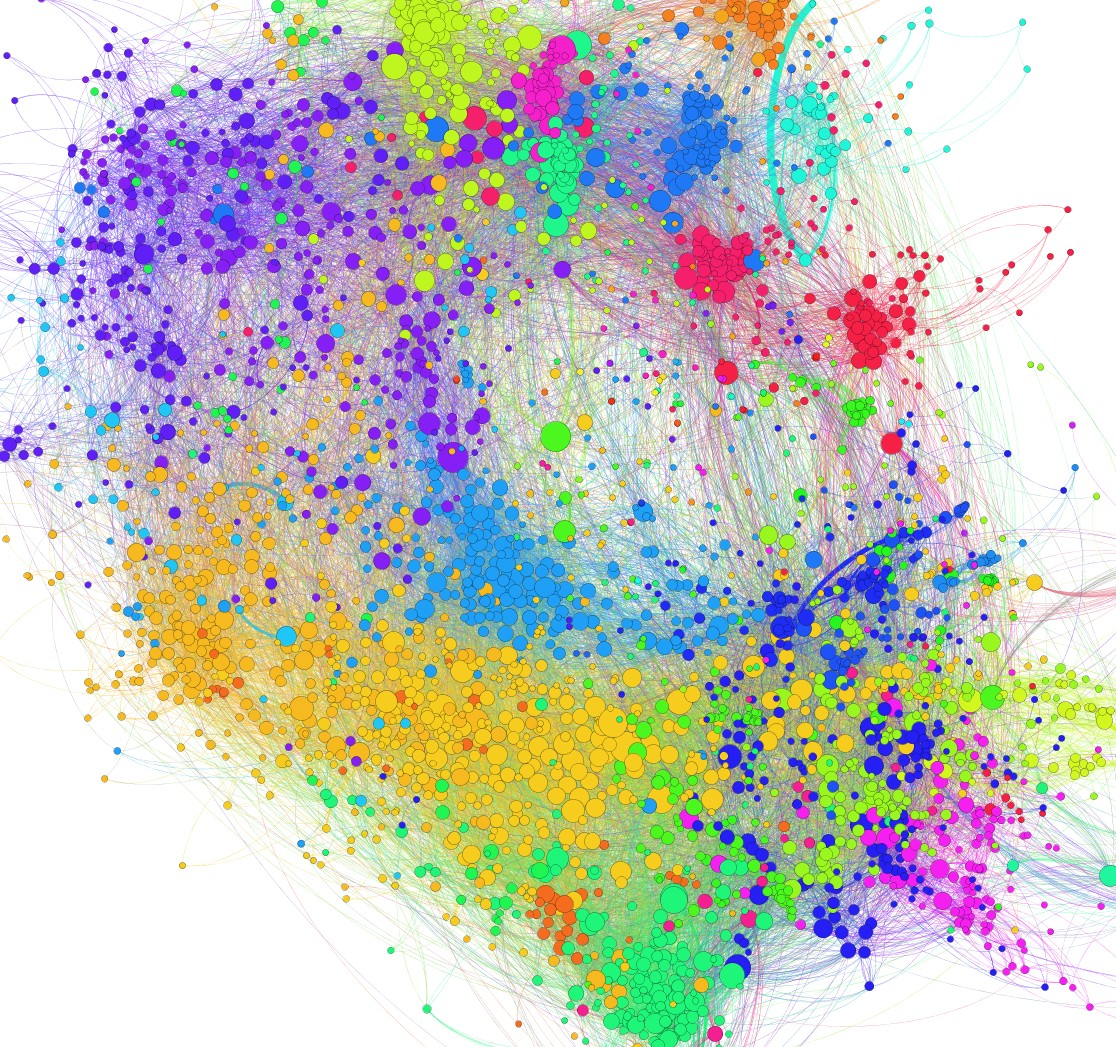
\includegraphics[width = 1.0 \textwidth, trim = 0 0 0 0cm , clip = true]
	{slides/Graph-screenshot.jpg}
	
\end{frame}

%%%%%%%%%%%%%%%%%%%%%%%%%%%%%%%%%%%%%%%%%%%%%%%%%%%%%%%%%%%%%%%%%%%%%%%%%%%%%%%%%%%%%%%%%%%%%%%%%%%%%%%%%%%%%
\begin{frame}{Mundo Sano Foundation}
	\begin{block}{ ... actively fighting  Chagas epidemic in Latin America }

	The purpose of this work is to support ongoing national health campaigns 
	by analyzing mobility information contained in Call Detail Records.  
%	Este trabajo propone un modelo que utiliza información de registros (logs) de llamados telefónicos
%	como forma de observar en qué regiones del país se espera encontrar una alta proporción de chagásicos.
	
	\bigskip
	Las migraciones humanas tienen un rol crucial en la diseminación de la enfermedad.
	
%	El espíritu es utilizar las comunicaciones para inferir migraciones,
%	y mediante éstas, estimar la prevalencia de la enfermedad en toda la Argentina.
%	
	\bigskip
	We strongly assume that long-term migrations are related to fluid communications with the past area of residence.
%	El modelo supone que una buena forma de detectar migraciones es viendo que existen fluidas comunicaciones con el lugar de or\'igen.
%	
%	\bigskip
%	Incluso antes de que existieran las computadoras.
%
	\end{block}
\end{frame}


%% HABLAR de pre trabajos en vih y malaria en el D4D? .
%	

%%%%%%%%%%%%%%%%%%%%%%%%%%%%%%%%%%%%%%%%%%%%%%%%%%%%%%%%%%%%%%%%%%%%%%%%%%%%%%%%%%%%%%%%%%%%%%%%%%%%%%%%%%%%
\begin{frame}{Mobile Phone Data}

% \begin{block}{Los datos: CDRs}

The argentinian and mexican datasets consist of \textbf{anonymized} call detail records (CDRs), each from one national telco. The former ranges 5 months of data whilst the latter 24.

%Nuestro conjunto de datos consiste en 5 meses de registros de llamados (CDRs) \textbf{anonimizados} de una compañía telefónica en la \textbf{Rep\'ublica Argentina}.

\medskip
Each call record consists of:
%Cada registro contiene:
\begin{itemize}
	\item Origin and destination users. 
	%Usuarios anonimizados de origen y destino de la llamada.
	\item ID of origin antenna.
	%ID de la antena telefónica usada por el remitente para la comunicación.  
	\item Start time and duration in seconds.
	%Tiempo de inicio y duración de la llamada.
\end{itemize}

\medskip
In all, each dataset has more than 9 billion geolocalized calls in each dataset. The population coverage of each telco is of 8 million and 2 million mobile lines for the argentinean and mexican datasets respectively.
%En total son m\'as de 9,000,000,000 llamados geolocalizados de 40,000,000 millones de l\'ineas celulares. % a las cuales analizaremos sus patrones de comunicaciones.

\medskip
The antenna datasets consists of more than five thousand geolocalized antennas.
%Contamos además con la lista de antenas celulares, con su correspondiente geolocalización (latitud y longitud).

% \end{block}
\end{frame}

%%%%%%%%%%%%%%%%%%%%%%%%%%%%%%%%%%%%%%%%%%%%%%%%%%%%%%%%%%%%%%%%%%%%%%%%%%%%%%%%%%%%%%%%%%%%%%%%%%%%%%%%%%%%
\section{Unveiling Chagas: Methodology}
%%%%%%%%%%%%%%%%%%%%%%%%%%%%%%%%%%%%%%%%%%%%%%%%%%%%%%%%%%%%%%%%%%%%%%%%%%%%%%%%%%%%%%%%%%%%%%%%%%%%%%%%%%%%
	
%%%%%%%%%%%%%%%%%%%%%%%%%%%%%%%%%%%%%%%%%%%%%%%%%%%%%%%%%%%%%%%%%%%%%%%%%%%%%%%%%%%%%%%%%%%%%%%%%%%%%%%%%%%%

%para el simposio recomiendo comentar toda la parte de las caracteristicas
\begin{frame}{Epidemiology of Chagas}
			Chagas is a disease caused by the \textit{trypanozoma cruzi} parasite
			 that extends through the American continent and, recently, some parts of Europe.
			%El Chagas es una enfermedad endémica de la zona del Gran Chaco.
			% y tambi\'en predominante en algunas comunidades que han migrado de esta zona. .
			
			\medskip  With over 65 million people exposed and endemic in more than 21 Latin American countries.
			%Esta zona comprende el norte y Wnoroeste de la Argentina
			%así como varios países limítrofes (Brasil, Bolivia, Paraguay, Perú).			
\end{frame}

%%%%%%%%%%%%%%%%%%%%%%%%%%%%%%%%%%%%%%%%%%%%%%%%%%%%%%%%%%%%%%%%%%%%%%%%%%%%%%%%%%%%%%%%%%%%%%%%%%%%%%%%%%%%
\begin{frame}{Epidemiology of Chagas}		
			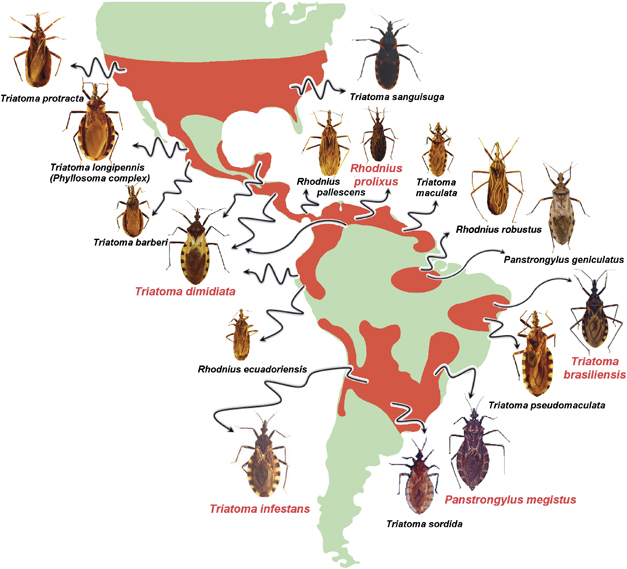
\includegraphics[height=.9\textheight]{slides/triatomine-map.jpg}
\end{frame}

%%%%%%%%%%%%%%%%%%%%%%%%%%%%%%%%%%%%%%%%%%%%%%%%%%%%%%%%%%%%%%%%%%%%%%%%%%%%%%%%%%%%%%%%%%%%%%%%%%%%%%%%%%%%
\begin{frame}{Epidemiology of Chagas}
	\begin{columns}		
		\begin{column}{0.45\textwidth}
			
			In Argentina, the disease is endemic in the \textit{Gran Chaco} region and
			also predominant in communities with migrations from this area.
			%El Chagas es una enfermedad endémica de la zona del Gran Chaco.
			% y tambi\'en predominante en algunas comunidades que han migrado de esta zona. .
			
			\medskip National estimates account for at least 1.5 million infected users and only 1 to 2 thousand
			treatments done yearly, where 30\% of all infected will develop a cardiopathy.
			% % % %DECIR ORAL: Seroprevalence tests in pregnant women reached 4.2% in 2009 which predicted 1.300 infected newborns that year.
			
		\end{column}
		\begin{column}{0.45\textwidth}
			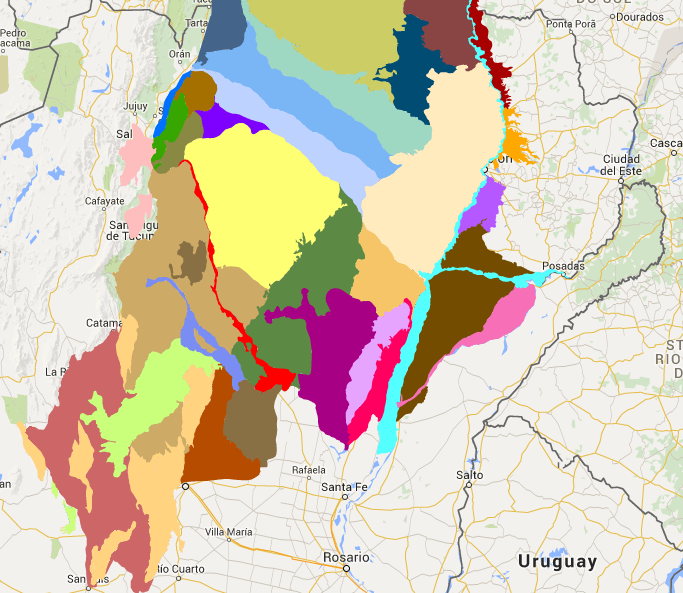
\includegraphics[height=.7\textheight]{slides/Ambientes_GranChaco_TNC-Argentina.png}
		\end{column}
	\end{columns}
\end{frame}

%%%%%%%%%%%%%%%%%%%%%%%%%%%%%%%%%%%%%%%%%%%%%%%%%%%%%%%%%%%%%%%%%%%%%%%%%%%%%%%%%%%%%%%%%%%%%%%%%%%%%%%%%%%%
\begin{frame}{Epidemiology of Chagas in Mexico}
	\begin{columns}
		\begin{column}{0.3\textwidth}
		
			In Mexico, the disease is endemic in some particular states of the country, shown in the map.
			%The disease is endemic in the states of Jalisco, Oaxaca, Veracruz, Guerrero, Morelos, Puebla, Hidalgo and Tabasco. 
			
			%This selection was based on the top 25\% prevalance states. 
			
			\medskip Non official reports estimate 5.5 million of potentially affected people and studies indicate that less than 0.5\% of infected have access to treatments. 

			% % % %DECIR ORAL: Seroprevalence tests in pregnant women reached 4.2% in 2009 which predicted 1.300 infected newborns that year.
		\end{column}
		\begin{column}{0.7\textwidth}
			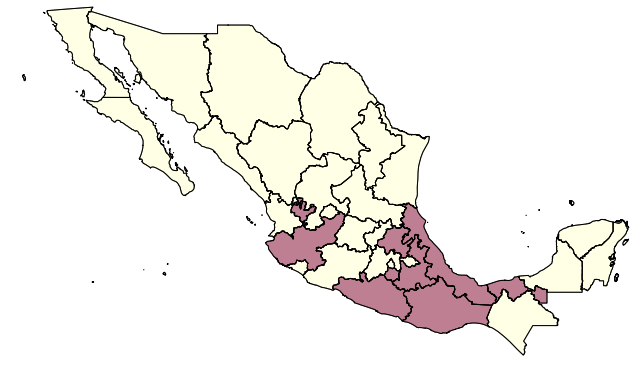
\includegraphics[width=\textwidth]{slides/Ambientes_Gran_Chaco-Mexico_original.png}
		\end{column}
	\end{columns}
\end{frame}
%%%%%%%%%%%%%%%%%%%%%%%%%%%%%%%%%%%%%%%%%%%%%%%%%%%%%%%%%%%%%%%%%%%%%%%%%%%%%%%%%%%%%%%%%%%%%%%%%%%%%%%%%%%%


\begin{frame}{Epidemiology of Chagas}
	Chagas is a disease:
	%El Chagas es una enfermedad:
	\begin{itemize}
		\item ... with different means of transmission and where long-term migrations play a key role. %explicar vertical, congenita y transfusion/transplante
		\item ... for which a low proportion of the infected population knows that they have the disease.
		\item ... whose asymptomatic phase can last more than 10 years.
		% % ORALLY SAY: 30 years of vector mitigation activities in GC. Current surveillance and control of the 
		\item ... which is epidemic and unattended.		 
	\end{itemize}
	%En particular, queremos encontrar chagásicos en zonas no tradicionalmente endémicas.
	%Es decir, gente de fuera de Gran Chaco infectada con \textit{Trypanosoma Cruzi} (el parásito que causa el Chagas).
\end{frame}

%%%%%%%%%%%%%%%%%%%%%%%%%%%%%%%%%%%%%%%%%%%%%%%%%%%%%%%%%%%%%%%%%%%%%%%%%%%%%%%%%%%%%%%%%%%%%%%%%%%%%%%%%%%%

%\begin{frame}{Objective: Chagas and Migrations}
%	Our goal is to find those traditionally non-endemic places which have most of the migratory exchange with the ecoregion. 
%	El objetivo es encontrar las zonas del país donde exista más intercambio migratorio con la zona del Gran Chaco.
%	
%	\bigskip
%	We aim to find infected people living in areas which are traditionally non-endemic.
%	Living outside \textit{Gran Chaco} and carrying the disease parasite \textit{trypanosoma cruzi} that causes Chagas.
%	
%	\medskip
%	Having a disease with long asymptomatic phases imply that long-term migrations are relevant to analyze.
%	
%	El período durante el cual se puede estar enfermo sin síntomas es tan alto
%	que se consideraron interesantes las migraciones largas.
%	
%	\medskip
%	
%	\begin{block}{The goal is to find...}
%		\begin{itemize}
%			\item individuals which have been infected in endemic areas and have later migrated.
%			gente que haya contraído la enfermedad en zonas endémicas y luego haya migrado.
%					\item ...personas que hayan nacido con ella (cuyos familiares/contactos pueden haber sido migrantes).	% Polémico? %naa
%			\item seasonal workers whose residence varies during the year. 
%			trabajadores golondrina, que cambien su residencia\\ de acuerdo a la estación del año.
%			\item outlying communities with probability of having a higher risk of Chagas prevalence.  
%			comunidades destacadas donde posiblemente exista una alta prevalencia de Chagas.
%		\end{itemize}
%	\end{block}
%	
%\end{frame}


%%%%%%%%%%%%%%%%%%%%%%%%%%%%%%%%%%%%%%%%%%%%%%%%%%%%%%%%%%%%%%%%%%%%%%%%%%%%%%%%%%%%%%%%%%%%%%%%%%%%%%%%%%%%
%%%%%%%%%%%%%%%%%%%%%%%%%%%%%%%%%%%%%%%%%%%%%%%%%%%%%%%%%%%%%%%%%%%%%%%%%%%%%%%%%%%%%%%%%%%%%%%%%%%%%%%%%%%%


%%%%%%%%%%%%%%%%%%%%%%%%%%%%%%%%%%%%%%%%%%%%%%%%%%%%%%%%%%%%%%%%%%%%%%%%%%%%%%%%%%%%%%%%%%%%%%%%%%%%%%%%%%%%
%%%%%%%%%%%%%%%%%%%%%%%%%%%%%%%%%%%%%%%%%%%%%%%%%%%%%%%%%%%%%%%%%%%%%%%%%%%%%%%%%%%%%%%%%%%%%%%%%%%%%%%%%%%%

% Procedimiento:
	% Obtener la lista de antenas de GC
	% Determinar la casa de los usuarios
	% Determinar, para cada usuario, si se comunicó con un habitante de GC
	% Determinar las agregaciones por antena
	% Visualizar(agrego alfa, min_volume y zoom en regiones)

\begin{frame}{Methodology (1)}
	
	\begin{block}{Home Prediction}
		\begin{itemize}
			\item As a first step, we determined each user's residence antenna. This was chosen to be the most used frequently used antenna during week evenings.
			%Como primer paso, determinamos para cada usuario, su lugar de residencia.
			 
			%La antena elegida como hogar es la más frecuentemente usada, 
			%considerando llamados nocturnos en días de semana.
			
			%\item The hypothesis: 
			%La hipótesis: la mayoría de los días, las personas se encuentran en sus casas durante la noche.
			
			%\bigskip
			%Así, cada antena queda asociada a un conjunto de usuarios: sus \textit{habitantes}.
			\item Users for which the inferred home antenna is located in an \textit{endemic area} will
			be considered the set of \textit{endemic users}. 
			%Nota: Los usuarios cuya antena inferida pertenece al Gran Chaco (la zona de riesgo)
			%se consideran el conjunto de \textit{habitantes de Gran Chaco}.
			
		\end{itemize}
	\end{block}
	\pause
	\begin{block}{Aggregation of vulnerable users}
		\begin{itemize}
			%\item For every user, we listed all of his call receivers in a given month.
			%Para cada usuario, obtuvimos la lista de todos los usuarios con los que se comunicó. %ojo que esto podria cambiar en versiones posteriores cuando cambie la definicion de 'vulnerable'
			
			\item If a given user communicated with the \textit{endemic area} in the selected period of time, we tagged him as potentially \textit{vulnerable}.

			%Si un usuario tuvo comunicaciones con la zona endémica (Gran Chaco), se considera que tiene mayor riesgo de tener Mal de Chagas, y lo marcamos como potentialmente \textit{vulnerable}.

			\item  We aggregated vulnerable users and total users (residents) per antenna.
			%Agregamos usuarios vulnerables y usuarios totales (habitantes) para cada antena.
			
			%\item We also aggregated the total volume of outgoing calls from every antenna and from these we extracted every call that had a user whose home is in the \textit{endemic area} as a receiver (\textit{vulnerable calls}).
			%Tambien agregamos el volumen total de llamados salientes de cada antena,
			%y de estos, los que tenían un habitante de Gran Chaco como destinatario (\textit{llamados vulnerables}).
			
			%\bigskip
			%Por lo tanto se obtuvieron, para cada antena, cuatro indicadores:
			%\begin{itemize}
			%	\item Cantidad de usuarios habitantes
			%	\item Cantidad de usuarios vulnerables entre los habitantes.
			%	\item Volumen de llamados salientes
			%	\item Volumen de llamados vulnerables salientes.
			%\end{itemize}
		\end{itemize}
	\end{block}
\end{frame}

%%%%%%%%%%%%%%%%%%%%%%%%%%%%%%%%%%%%%%%%%%%%%%%%%%%%%%%%%%%%%%%%%%%%%%%%%%%%%%%%%%%%%%%%%%%%%%%%%%%%%%%%%%%%
\begin{frame}{Methodology (2)}
	
	
	\begin{block}{Mapas de calor}
		
		
		We generated heat maps from these results, plotting a colored circle around each antenna, which encodes its \textit{vulnerable} communication patterns.
		%A partir de los datos obtenidos, generamos mapas de calor que representan las comunicaciones de la celda con el Gran Chaco.
		
		% DECIR: en este trabajo encnotramos areas de alta interaccion con lazona endemica a traves de analizar los mapas de calor entre ls residentes de una zona con otra.
			
		%Generamos un c\'irculo por cada celda donde:
		\begin{itemize}
			\item the \textbf{area} depends on the on the volume of use.
			%el \textbf{\'area} depende de la cantidad de usuarios (habitantes),
			\item the \textbf{color} corresponds to the percentage of vulnerable use in that antenna (whether calls or users).
			%el \textbf{color} corresponde al porcentaje de usuarios vulnerables que viven en esa antena.
		\end{itemize}
		
	\end{block}
	
	\begin{block}{Antenna Filter}
		$\beta$ will be our parameter to filter antennas by minimum vulnerable interaction rates. 
%		We added two filtering thresholds $\beta$ and $min\_volumen$ which will control the antennas to be plotted if the percentage and volume of vulnerable interactions for that cell are higher than their respective thresholds.
		%Every antenna will be plotted if:
		% Notar que en ningún lado antes de esto dijimos que íbamos a pintar un mapa de Argentina con las antenas.
		%Dos par\'ametros $\beta$ y $min\_volumen$  filtran la lista de antenas a ser visualizadas.
		%Cada antena se grafica si:
		%\begin{itemize}
		%	\item the percentage of vulnerable users/calls is bigger than  $\beta$.
			%el porcentaje de usuarios vulnerables es mayor que $\beta$,
		%	\item the volume of vulnerable users/calls is bigger than $min\_volumen$. 
			%el volumen de uso vulnerable es mayor que $min\_volumen$ de llamados o usuarios.
		%\end{itemize}
		
		%
		%\bigskip
		%Por lo tanto, el modelo permitiría ver las antenas donde existen mayores lazos familiares con el Gran Chaco.	% Creo que 'familiares' es muy fuerte
		
		%\bigskip
		%A\'un con los par\'ametros anteriores, fue necesario separar el filtrado por distintas regiones:
		%
		%\smallskip
		%Una antena de baja proporción a nivel nacional ($\beta=10\%$) puede ser llamativa, por ejemplo, en Tierra del Fuego.
		%%aca se inserta imagen x ejemplo?? %No, la imagen es demasiado grande me parece. Lo podemos discutir.
		
	\end{block}
\end{frame}

%%%%%%%%%%%%%%%%%%%%%%%%%%%%%%%%%%%%%%%%%%%%%%%%%%%%%%%%%%%%%%%%%%%%%%%%%%%%%%%%%%%%%%%%%%%%%%%%%%%%%%%%%%%%
\section{Exploración de los datos}
%%%%%%%%%%%%%%%%%%%%%%%%%%%%%%%%%%%%%%%%%%%%%%%%%%%%%%%%%%%%%%%%%%%%%%%%%%%%%%%%%%%%%%%%%%%%%%%%%%%%%%%%%%%%



%%%%%%%%%%%%%%%%%%%%%%%%%%%%%%%%%%%%%%%%%%%%%%%%%%%%%%%%%%%%%%%%%%%%%%%%%%%%%%%%%%%%%%%%%%%%%%%%%%%%%%%%%%%%
\begin{frame}
	\frametitle{Mapa de calor: Argentina, $\beta$ = 1 \%}
	\center
	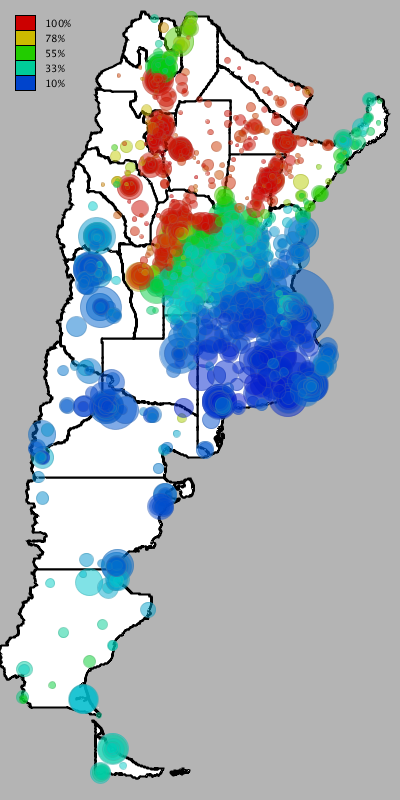
\includegraphics[height=.9\textheight,width = .9\columnwidth, keepaspectratio]
	{slides/201112_hi_res_argentina_usuarios_proporcion_circulos_beta1.png}
\end{frame}

%%%%%%%%%%%%%%%%%%%%%%%%%%%%%%%%%%%%%%%%%%%%%%%%%%%%%%%%%%%%%%%%%%%%%%%%%%%%%%%%%%%%%%%%%%%%%%%%%%%%%%%%%%%%
\begin{frame}
	\frametitle{Mapa de calor: Argentina, $\beta$ = 15 \%}
	\center
	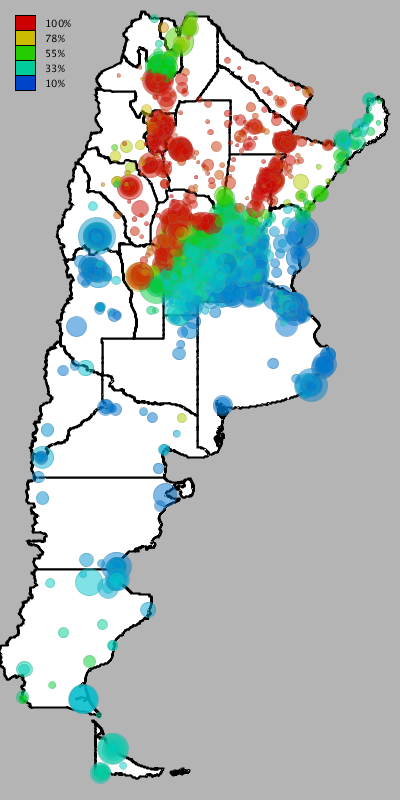
\includegraphics[height=.9\textheight,width = .9\columnwidth, keepaspectratio]
	{slides/201112_hi_res_argentina_usuarios_proporcion_circulos_beta15.png}
\end{frame}

%%%%%%%%%%%%%%%%%%%%%%%%%%%%%%%%%%%%%%%%%%%%%%%%%%%%%%%%%%%%%%%%%%%%%%%%%%%%%%%%%%%%%%%%%%%%%%%%%%%%%%%%%%%%
\begin{frame}
	\frametitle{Mapa de calor: Argentina, $\beta$ = 30 \%}
	\center
	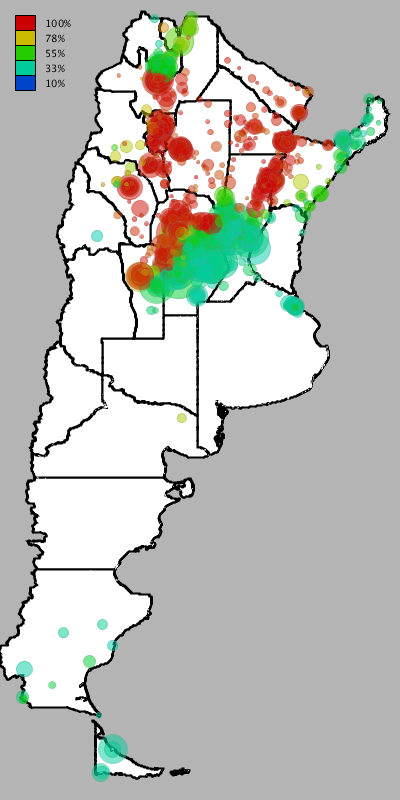
\includegraphics[height=.9\textheight,width = .9\columnwidth, keepaspectratio]
	{slides/201112_hi_res_argentina_usuarios_proporcion_circulos_beta30.png}
\end{frame}

%%%%%%%%%%%%%%%%%%%%%%%%%%%%%%%%%%%%%%%%%%%%%%%%%%%%%%%%%%%%%%%%%%%%%%%%%%%%%%%%%%%%%%%%%%%%%%%%%%%%%%%%%%%%
\begin{frame}
	\frametitle{Mapa de calor: Argentina, $\beta$ = 50 \%}
	\center
	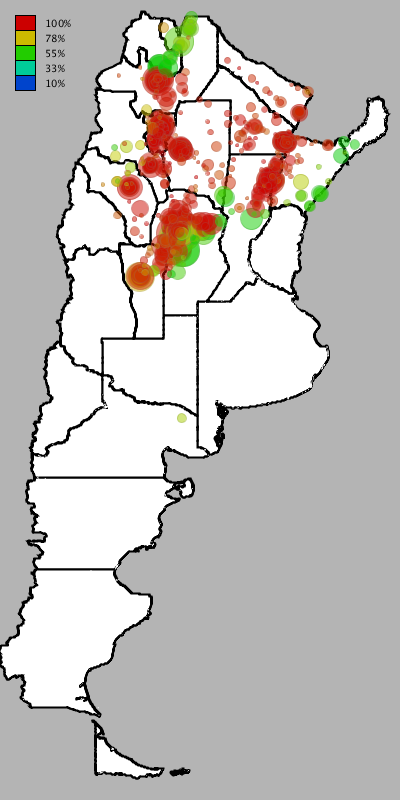
\includegraphics[height=.9\textheight,width = .9\columnwidth, keepaspectratio]
	{slides/201112_hi_res_argentina_usuarios_proporcion_circulos_beta50.png}
\end{frame}

%%%%%%%%%%%%%%%%%%%%%%%%%%%%%%%%%%%%%%%%%%%%%%%%%%%%%%%%%%%%%%%%%%%%%%%%%%%%%%%%%%%%%%%%%%%%%%%%%%%%%%%%%%%%

\setbeamercolor{background canvas}{bg=white}

\begin{frame}{Regiones focalizadas}
	A partir de estas primeras visualizaciones, con la gente de la fundación decidimos focalizar la granularidad en regiones específicas y fuera del Gran Chaco.
	%A partir de estos primeros mapas se decidi\'o enfocar la visualizaci\'on y mejorar la precisi\'on en ciertas regiones fuera del Gran Chaco. 
		\begin{itemize}
			\item Tierra del Fuego
			\item Este de R\'io Negro
			\item Buenos Aires
			\item Capital Federal, South and North CABA, and AMBA
			\item C\'ordoba Central 
		\end{itemize}		
\end{frame}

%%%%%%%%%%%%%%%%%%%%%%%%%%%%%%%%%%%%%%%%%%%%%%%%%%%%%%%%%%%%%%%%%%%%%%%%%%%%%%%%%%%%%%%%%%%%%%%%%%%%%%%%%%%%
\begin{frame}
	\frametitle{Mapa de calor: AMBA, $\beta$ = 2 \%}
	\centering
	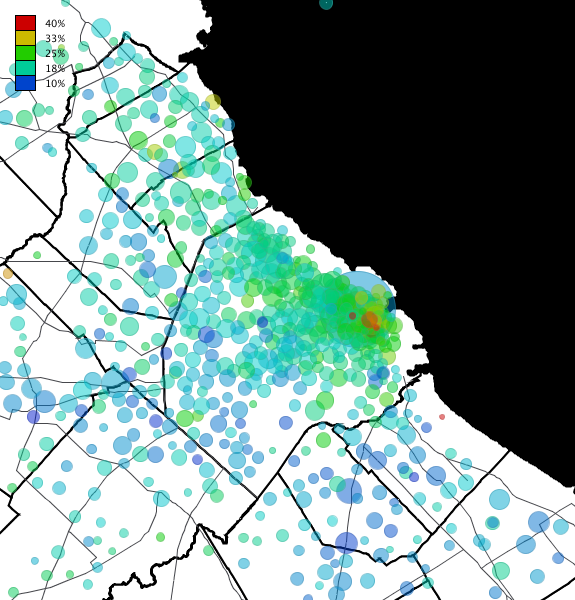
\includegraphics[height=.9\textheight,width = .9\columnwidth,keepaspectratio]
	{slides/201112_hi_res_amba_usuarios_proporcion_circulos_beta2.png}
\end{frame}
%%%%%%%%%%%%%%%%%%%%%%%%%%%%%%%%%%%%%%%%%%%%%%%%%%%%%%%%%%%%%%%%%%%%%%%%%%%%%%%%%%%%%%%%%%%%%%%%%%%%%%%%%%%%
\begin{frame}
	\frametitle{Mapa de calor: AMBA, $\beta$ = 10 \%}
	\centering
	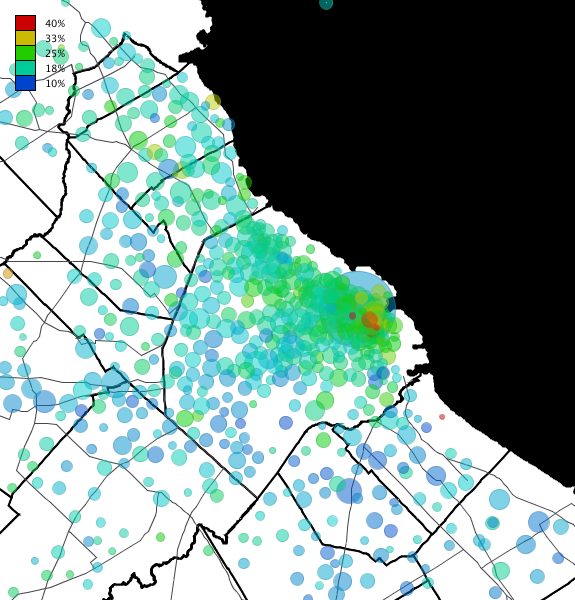
\includegraphics[height=.9\textheight,width = .9\columnwidth,keepaspectratio]
	{slides/201112_hi_res_amba_usuarios_proporcion_circulos_beta10.png}
\end{frame}
%%%%%%%%%%%%%%%%%%%%%%%%%%%%%%%%%%%%%%%%%%%%%%%%%%%%%%%%%%%%%%%%%%%%%%%%%%%%%%%%%%%%%%%%%%%%%%%%%%%%%%%%%%%%
\begin{frame}
	\frametitle{Mapa de calor: AMBA, $\beta$ = 20 \%}
	\centering
	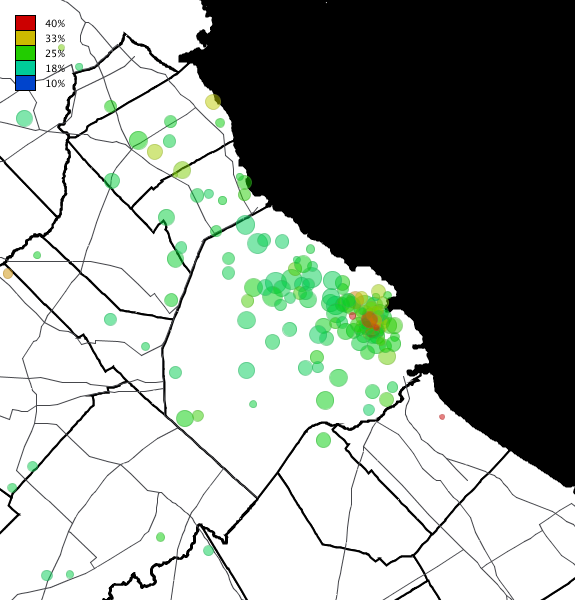
\includegraphics[height=.9\textheight,width = .9\columnwidth,keepaspectratio]
	{slides/201112_hi_res_amba_usuarios_proporcion_circulos_beta20.png}
\end{frame}
%%%%%%%%%%%%%%%%%%%%%%%%%%%%%%%%%%%%%%%%%%%%%%%%%%%%%%%%%%%%%%%%%%%%%%%%%%%%%%%%%%%%%%%%%%%%%%%%%%%%%%%%%%%%
\begin{frame}
	\frametitle{Heat Map AMBA, $\beta$ = 28 \%}
	\centering
	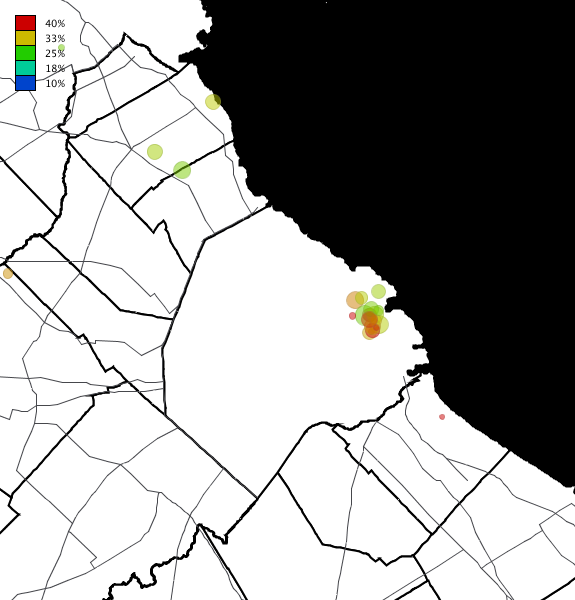
\includegraphics[height=.9\textheight,width = .9\columnwidth,keepaspectratio]
	{slides/201112_hi_res_amba_usuarios_proporcion_circulos_beta28.png}
\end{frame}
%%%%%%%%%%%%%%%%%%%%%%%%%%%%%%%%%%%%%%%%%%%%%%%%%%%%%%%%%%%%%%%%%%%%%%%%%%%%%%%%%%%%%%%%%%%%%%%%%%%%%%%%%%%%

\begin{frame}{Argentine Communities Detected}
	After filtering the maps, we are left with few antennas that stick out for their risk level. Using their location, we assign them to Argentinian communities or cities. 
	
	%Como resultado del filtrado en cada zona, nos hemos quedado con las antenas destacadas por su nivel de riesgo y, utilizando su ubicaci\'on, las emparejamos con localidades o comunidades argentinas. 
	
	\bigskip
	
	\begin{block}{Some communities outside the big cities}
		\begin{itemize}
			\item Cordoba: Freyre, La Tordilla, Balnearia, ... % etc. %hay muchas mas pero no se si esta bien poner esto
			\item AMBA: Avellaneda, Parque Patricios, San Isidro, ... % etc.
			\item Bs As Province: Lima, San Nicolas.
			\item La Rioja: Chamical and Malanz\'an.
			\item Salta: Tartagal.
		\end{itemize}
		
	\end{block}
\end{frame}

%%%%%%%%%%%%%%%%%%%%%%%%%%%%%%%%%%%%%%%%%%%%%%%%%%%%%%%%%%%%%%%%%%%%%%%%%%%%%%%%%%%%%%%%%%%%%%%%%%%%%%%%%%%%
%\begin{frame}{Ongoing Tasks}
		
%	{\Large Enrich antenna data with epidemic risk factors and segmenting for:}
	% %SAY ORALLY: filter communications for non working schedules. Try to see if any pattern occurs at a smaller scale since which would add insight to the analysis or become an interesting feature.
%	\begin{itemize}
%		\item Rural locations. % etc. %hay muchas mas pero no se si esta bien poner esto
%		\item Housing conditions. % etc.
%	\end{itemize}
	% %SAY ORALLY: Focus the communications analysis on communities where Mundo Sano is currently working 
		
%%%%%%%%%%%%%%%%%%%%%%%%%%%%%%%%%%%%%%%%%%%%%%%%%%%%%%%%%%%%%%%%%%%%%%%%%%%%%%%%%%%%%%%%%%%%%%%%%%%%%%%%%%%%
\section{Prediction of Long-term Mobility}
%%%%%%%%%%%%%%%%%%%%%%%%%%%%%%%%%%%%%%%%%%%%%%%%%%%%%%%%%%%%%%%%%%%%%%%%%%%%%%%%%%%%%%%%%%%%%%%%%%%%%%%%%%%%
\begin{frame}{Mobility Classifier}
%	\begin{columns}
%		\begin{column}{0.20 \textwidth}
			\begin{block}{Target Variable}
			Let $T_0$ and $T_1$ be time periods corresponding to $($01/01/14, 31/07/15 $)$ and $($01/08/15, 31/12/15$)$ respectively.
			
			Consider $U_0$ to be the set of users that lived in the \textbf{mexican} endemic region $E_Z$ during period $T_0$. Then our target variable $Y$ for every user $u$ is:  
			\[
			%\begin{equation}
			Y_u =
			\begin{cases}
			&1 \ \mbox{if} \ u \in U_0  \\
			&0 \ \mbox{in other cases}.
			\end{cases}
			%\end{equation}
			\]
			where $\ u \in U_0$ iff the user's home antenna is in $E_Z$ during $T_0$.
			\end{block}
	
\end{frame}

%%%%%%%%%%%%%%%%%%%%%%%%%%%%%%%%%%%%%%%%%%%%%%%%%%%%%%%%%%%%%%%%%%%%%%%%%%%%%%%%%%%%%%%%%%%%%%%%%%%%%%%%%%%%
\begin{frame}{Feature Matrix Description}
	The features were constructed using data during the period $T_0$ and amount to a total of 130 variables per user.
	
	\begin{itemize}
		\item Volume of ten most used antennas.
		\item Mobility diameter.
		%Presentamos una utilizaci\'on novedosa de los CDRs (Call Detail Records), datos que
		%fueron recogidos para otro fin (facturación). 
		\item Graph data and communications, segmented accordingly:
		\begin{itemize}
			\item Month of interaction.
			\item Time of the week.
			\item Vulnerability of the interactions.
			\item Duration, volume and direction of the interactions.
		\end{itemize}
	\end{itemize}
	
	\begin{block}{Feature - Target Correlation}
		
	As expected, there was a high Pearson correlation between $Y$ and calling patterns with the endemic region. 
	%All of them being above \($0.7$\). 
	\end{block}
		
\end{frame}

%%%%%%%%%%%%%%%%%%%%%%%%%%%%%%%%%%%%%%%%%%%%%%%%%%%%%%%%%%%%%%%%%%%%%%%%%%%%%%%%%%%%%%%%%%%%%%%%%%%%%%%%%%%%

\begin{frame}{ ML setup}

%		\begin{block}{ML Setup}
			
			Standard industry classifiers were fit with
			and 5-Fold cross validation and a 10\% hold out set for scoring.
			
			\medskip
			
			All standard metrics used rated higher than $0.96$. The lowest of them being the weighted F1 score with $0.964$.
%		\end{block}
		
%		
%		\begin{block}{Scores}					
%			 					
%		\end{block}
%
		
\end{frame}

%%%%%%%%%%%%%%%%%%%%%%%%%%%%%%%%%%%%%%%%%%%%%%%%%%%%%%%%%%%%%%%%%%%%%%%%%%%%%%%%%%%%%%%%%%%%%%%%%%%%%%%%%%%%
\section{Conclusion}
%%%%%%%%%%%%%%%%%%%%%%%%%%%%%%%%%%%%%%%%%%%%%%%%%%%%%%%%%%%%%%%%%%%%%%%%%%%%%%%%%%%%%%%%%%%%%%%%%%%%%%%%%%%%

%%%%%%%%%%%%%%%%%%%%%%%%%%%%%%%%%%%%%%%%%%%%%%%%%%%%%%%%%%%%%%%%%%%%%%%%%%%%%%%%%%%%%%%%%%%%%%%%%%%%%%%%%%%%
% Conclusiones:
% Los mapas de calor reflejean los esperado respecto al "gradiente" de calor.
% Re-utilizacion de logs para otro uso, uso novedoso. Barato y simple, agarrar datos que existen y se reinterpretan.
% Posible herramienta para buscar infectados en otras enfermedades donde tambien existen zonas endemicas y prevalencia en el tiempo de la enfermedad.
\begin{frame}{Conclusions}
	\begin{block}{Expected}
		Heat maps show \textit{temperature} falling from \textbf{Gran Chaco} outwards; heat that descents rapidly as we move away from the area.
		
		\medskip
		The assumption used to build the heatmaps were confirmed on the mexican dataset, with high feature correlation to past residence.
		
	\end{block}
	
	\pause
	
	\begin{block}{Unexpected}		
		Non-homogeneous communication patterns with the ecoregion allowed us to find outlying communities that stick out for their high link with the studied region.
		
		\medskip
		The maps provide a tool to \textbf{prioritize screening campaigns for Chagas Disease}.
		
		\medskip
		High scoring classifiers.
	\end{block}
\end{frame}

%%%%%%%%%%%%%%%%%%%%%%%%%%%%%%%%%%%%%%%%%%%%%%%%%%%%%%%%%%%%%%%%%%%%%%%%%%%%%%%%%%%%%%%%%%%%%%%%%%%%%%%%%%%%
%%%%%%%%%%%%%%%%%	
	
\begin{frame}{Conclusions}
	\begin{block}{CDR Reuse}
		\begin{itemize}
			\item Novel use for CDRs which is originally logged for other purposes (billing).
			%Presentamos una utilizaci\'on novedosa de los CDRs (Call Detail Records), datos que
			%fueron recogidos para otro fin (facturación).
			\item Low-cost and potentially of high-value.
			%El análisis de datos existentes tiene bajo costo y potentialmente mucho valor.
			\item Can be extended to other regions or diseases and epidemics of similar characteristics.
			%Prueba de concepto que se puede extender a enfermedades y epidemias de caracter\'isticas similares.
		\end{itemize}
		
		
	\end{block}
\end{frame}

%%%%%%%%%%%%%%%%%%%%%%%%%%%%%%%%%%%%%%%%%%%%%%%%%%%%%%%%%%%%%%%%%%%%%%%%%%%%%%%%%%%%%%%%%%%%%%%%%%%%%%%%%%%%
%%%%%%%%%%%%%%%%%

%\begin{frame}{Future Work - RETOCAR}
%
%		\begin{block}{Enhance the Communications Model}
%			\begin{itemize}
%			\item Current vulnerability characterization relies exclusively on mobile communications of users with antennas in the ecoregion.
%			%La caracterizaci\'on actual de la vulnerabilidad viene dada por contacto telefónicos con usuarios de antenas del Gran Chaco. 
%			
%			\item We look forward to extracting long-term mobility information by looking at communication patterns between two areas.
%			% %SAY ORALLY: Focus the communications analysis on communities where Mundo Sano is currently working 
%			\end{itemize}
%  	 	\end{block}
% \end{frame}
%  	 		
  
  %%%%%%%%%%%%%%%%%%%%%%%%%%%%%%%%%%%%%%%%%%%%%%%%%%%%%%%%%%%%%%%%%%%%%%%%%%%%%%%%%%%%%%%%%%%%%%%%%%%%%%%%%%%%
  
%   \begin{frame}{Future Work}
%   	
%\begin{block}{New Data Sources (if available)}
%	 With Mundo Sano we aim to incorporate epidemiological data to the analysis:
%\begin{itemize}
%\item tenement bug infestation
%\item infected rates by municipality 
%\item infected newborns
%\item acute Chagas cases.
%\item serological data per community, amongst others.
%\end{itemize}
%
%\end{block}
%
%\begin{block}{2010 Census}
%	Socio-economic information aggregated by department from the national census website \footnote{ http://censo2010.indec.gov.ar/} has already been preprocessed for every municipality in Argentina.
%	
%	 
%	
%\end{block}
%   \end{frame}
%   




%%%%%%%%%%%%%%%%%%%%%%%%%%%%%%%%%%%%%%%%%%%%%%%%%%%%%%%%%%%%%%%%%%%%%%%%%%%%%%%%%%%%%%%%%%%%%%%%%%%%%%%%%%%%
% ==============================================

\begin{frame}{Thank you! $:)$}
	\begin{columns}
		\begin{column}{0.20 \textwidth}
		\end{column}
		
		\begin{column}{0.55 \textwidth}
			
			\begin{block}{Questions?}
				\center
				Juan de Monasterio \\
				\textit{laterio@gmail.com} \\
				\bigskip
				Carolina Lang \\
				\textit{carolinalang93@gmail.com} \\
				\bigskip				
				Carlos Sarraute \\
				\textit{charles@grandata.com} \\
				
				
			\end{block}
		\end{column}
		\begin{column}{0.20 \textwidth}
		\end{column}
	\end{columns}
	
\end{frame}


% ==============================================

\justifying%
\scalefont{0.7}
\bibliographystyle{unsrtnat}
\bibliography{../mobility}

% \end{columns}

% ==============================================

\vfill


\end{document}

